\section{Design and Architecture}
\subsection{Design and Architecture}
\begin{frame}{Design and Architecture}
\begin{itemize}
    \item<1-> The following shows an overview of how ForkPi and SpoonPi are setup.
    \item<2-> 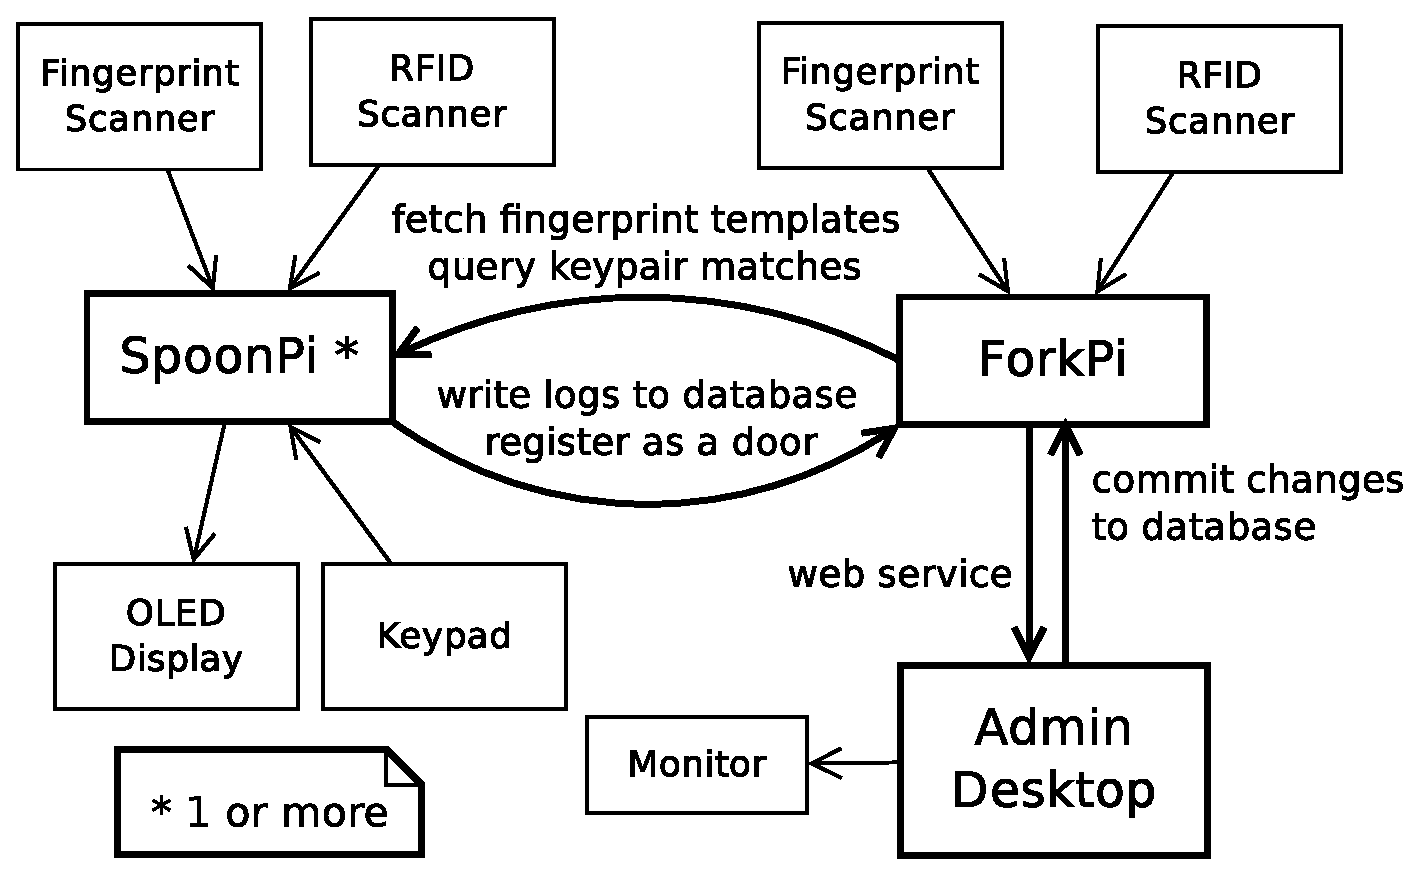
\includegraphics[scale=0.5]{architecture.eps}
\end{itemize}
\end{frame}

\subsection{ForkPi}
\begin{frame}{ForkPi Overview}
\begin{itemize}
    \item<1-> The ForkPi unit functions as both a web and database server.
    \item<2-> The web server runs a locally accessible website where one can register new users into the system, view logs, and perform other administrative actions.
    \item<3-> The web server has an underlying database run by PostgreSQL.
    \item<4-> Human administrators view ForkPi as a web server, while SpoonPis view ForkPi as a database server.
\end{itemize}
\end{frame}

\begin{frame}{Technical Overview}
\begin{itemize}
    \item<1-> ForkPi is addressed within the local network using the name forkpi.local, at HTTP port 80.
    \item<2-> The database server runs in the port 5432, so SpoonPis will access the database using the host name forkpi.local and the port number 5432.
    \item<3-> A dedicated ForkPi unit does not require the presence of a keypad nor an OLED display, but it requires having the following peripherals attached:
    \begin{itemize}
    	\item<4-> \textbf{RFID Scanner}: for scanning the UIDs of RFID tags to be registered
		\item<5-> \textbf{Fingerprint Scanner}: for the enrollment of new Fingerprints
    \end{itemize}
\end{itemize}
\end{frame}

\begin{frame}{Use Case Diagram}
\begin{itemize}
    \item<1-> 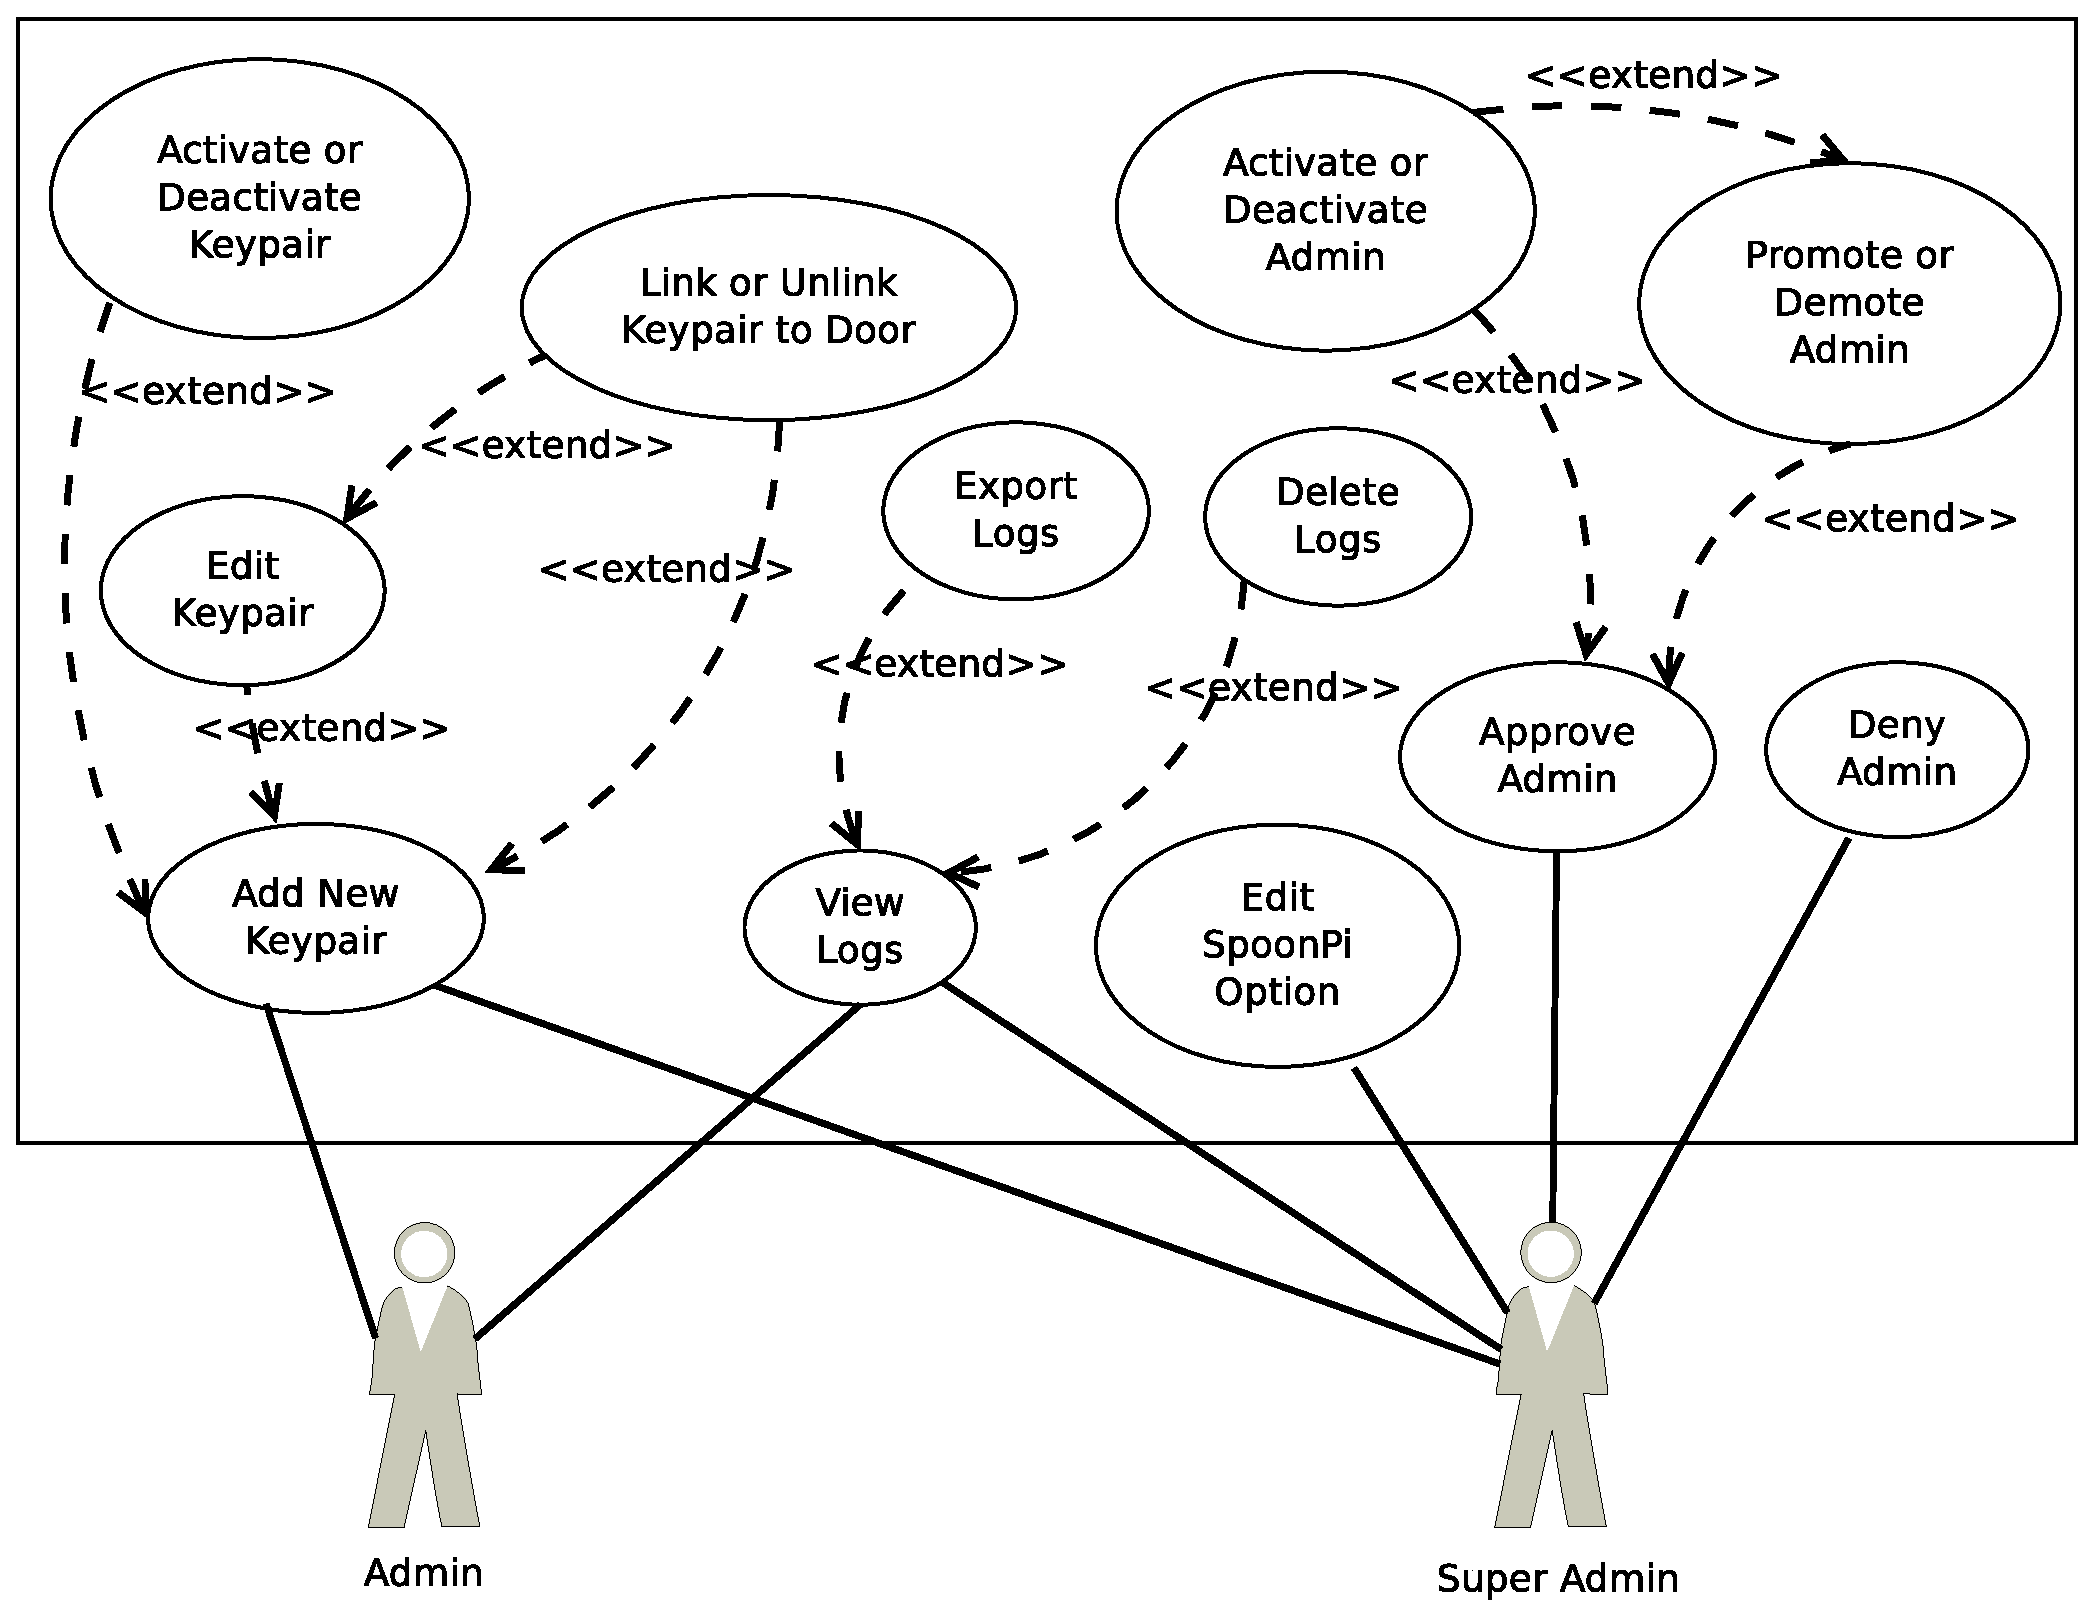
\includegraphics[scale=0.3]{forkpi-use-case.eps}
\end{itemize}
\end{frame}

\begin{frame}{Types of Admins}
\begin{itemize}
    \item<1-> There are two types of admins: regular admins and super admins.
    \item<2-> Super admins can perform everything a regular admin can do, with some additional functions we deemed to be potentially destructive in the hands of the wrong person. %% *SUCH AS???
    \item<3-> Regular admins have a limited set of permissions, and they can only become super admins with the consent of another super admin, in a process called promotion.
    \item<4-> New admin sign up requires the approval of another admin, and is a regular admin by default.
    \item<5-> However, if the system is new, admin sign up is automatically approved and is a super admin by default.
\end{itemize}
\end{frame}

\subsection{SpoonPi}
\begin{frame}{SpoonPi Overview}
\begin{itemize}
    \item<1-> The SpoonPi units serve as the media for door authentication, and are responsible for granting or denying access through doors. There are as many SpoonPis as doors to be secured.
    \item<2-> Each SpoonPi unit needs to register itself first with the ForkPi unit before any authentication can be done.
    \item<3-> SpoonPi performs authentication by communicating with the hardware components (e.g. RFID scanner) to get the input credentials (e.g. RFID UID), then querying the ForkPi database to check if it is valid.
    \item<4-> For fingerprint authentication, the verification is done at the SpoonPi side instead of the ForkPi side, because the matching is not a simple string comparison; fingerprint templates have to be uploaded to the scanner, where the actual matching takes place.
\end{itemize}
\end{frame}

\begin{frame}{Technical Overview}
\begin{itemize}
    \item<1-> A SpoonPi unit requires having the following peripherals attached:
    \begin{itemize}
    	\item<2-> \textbf{Fingerprint Scanner}: for identifying the fingerprint presented
		\item<3-> \textbf{OLED}: for displaying the current status of the transaction
		\item<4-> \textbf{RFID} Scanner: for scanning the UID of the RFID tag presented
		\item<5-> \textbf{Keypad}: for entering the PIN
    \end{itemize}
\end{itemize}
\end{frame}

\begin{frame}{SpoonPi Flowchart}
\begin{itemize}
    \item<1-> The following flowchart describing the main transaction loop:
    \item<2-> 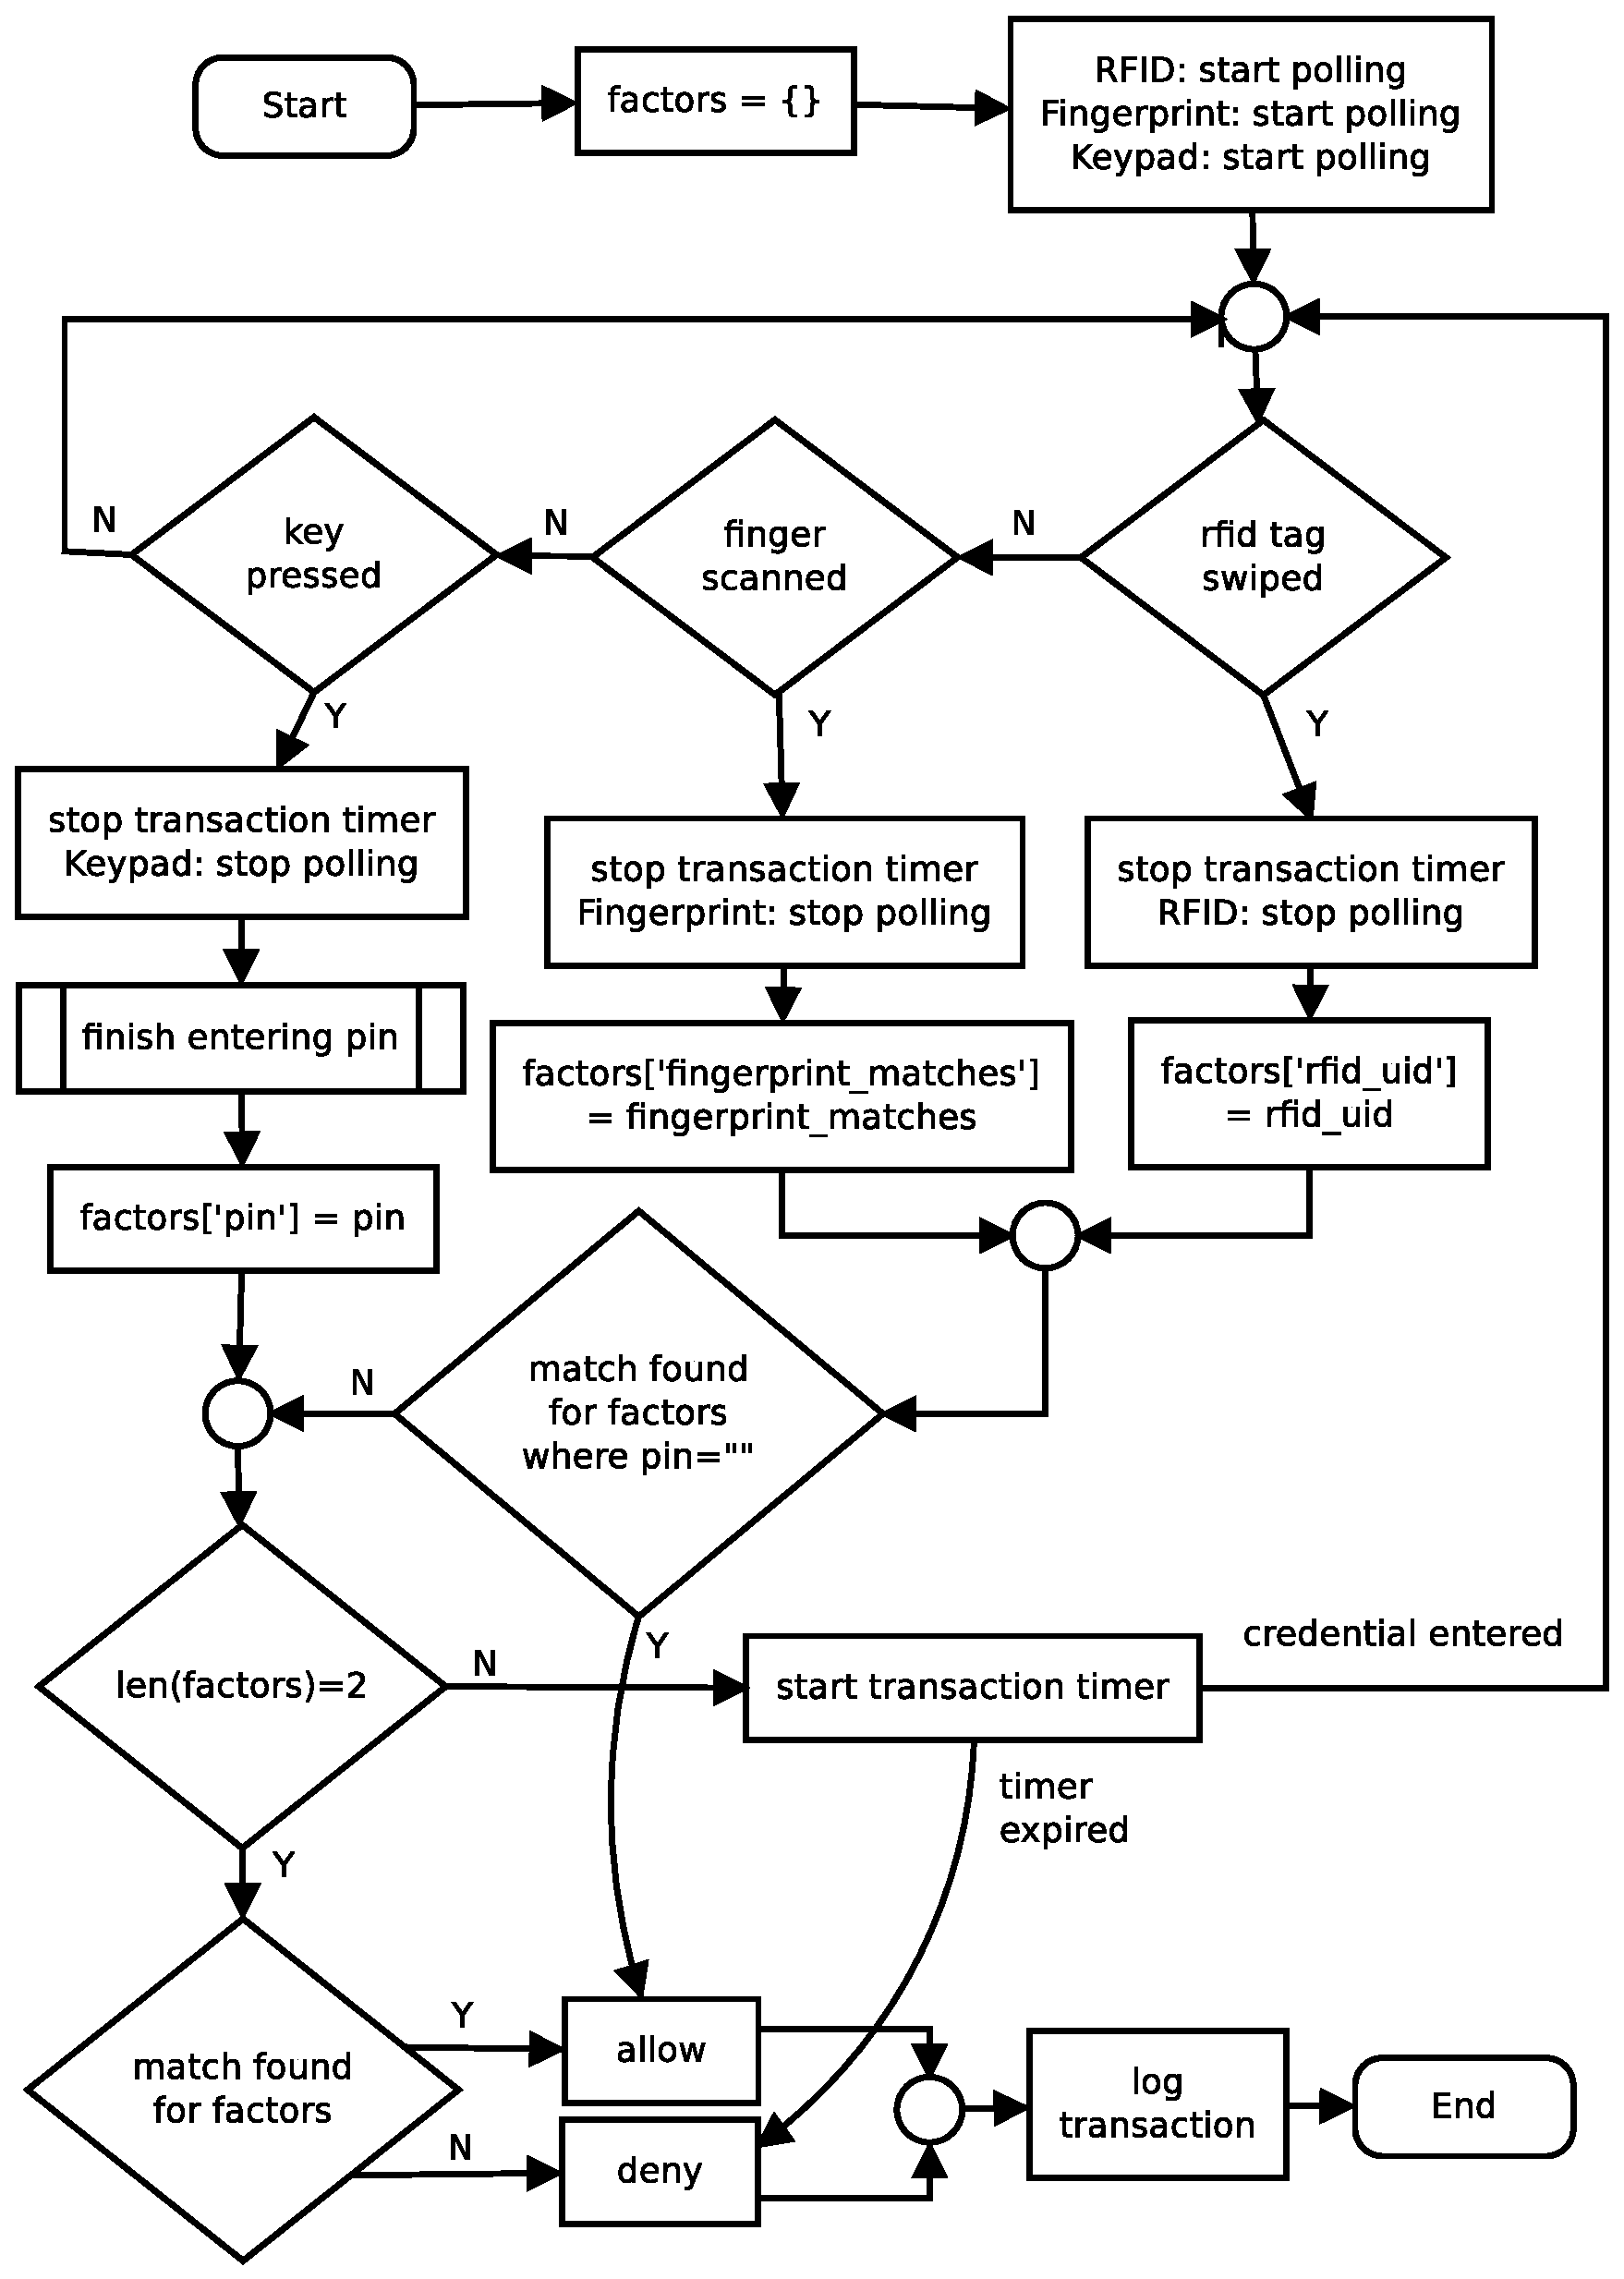
\includegraphics[scale=0.2]{spoonpi-flowchart.eps}
\end{itemize}
\end{frame}

\begin{frame}{SpoonPi PIN Flowchart}
\begin{itemize}
    \item<1-> The following flowchart describing the PIN input loop:
    \item<2-> 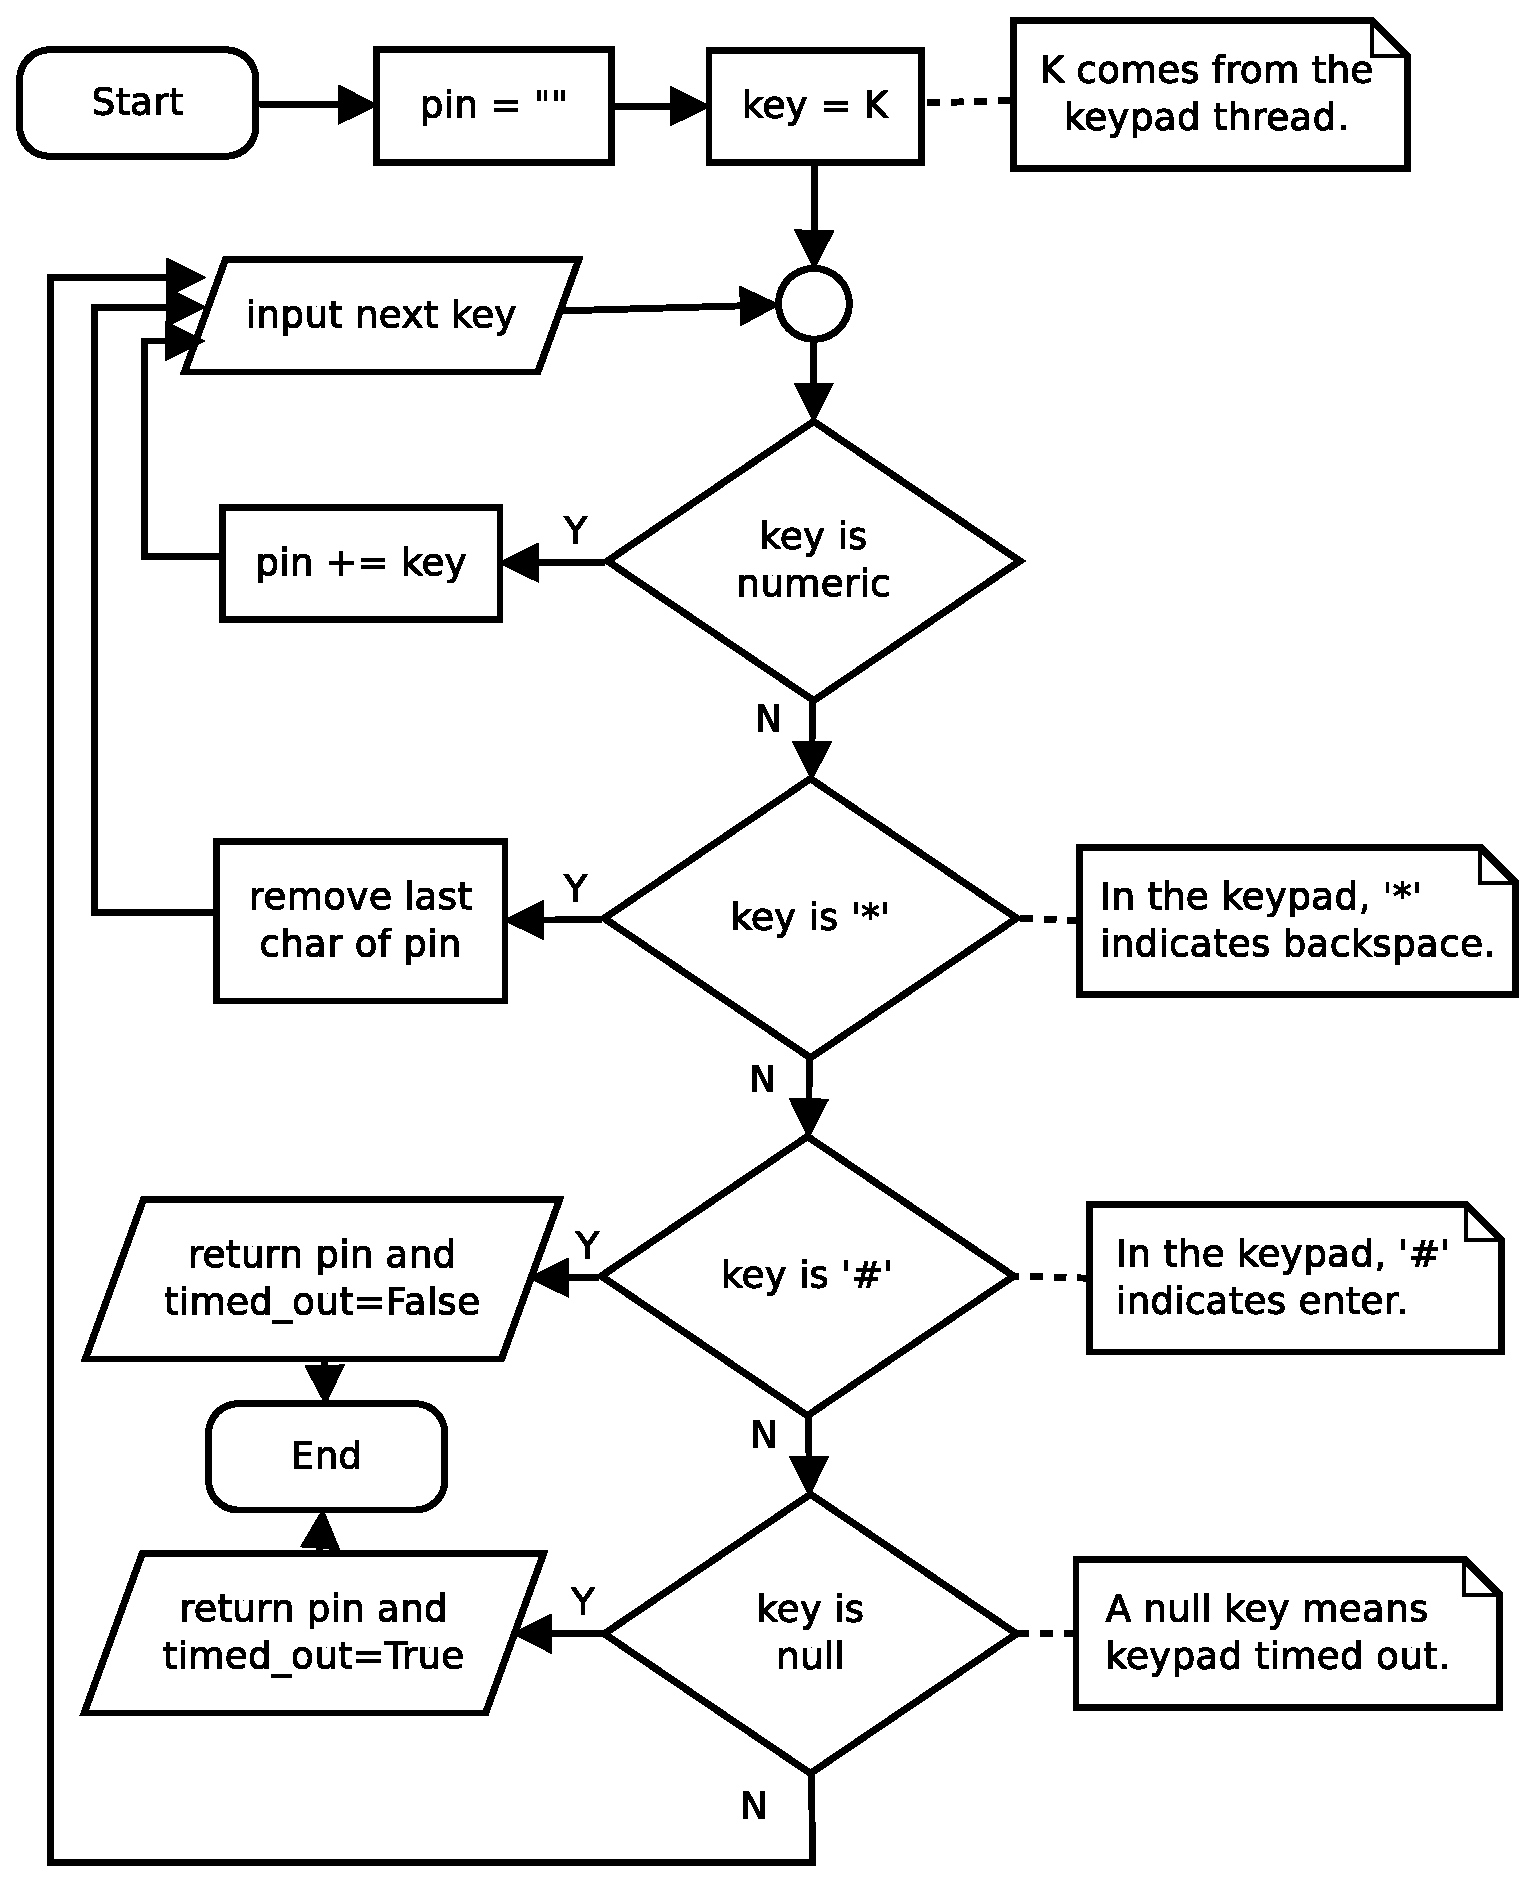
\includegraphics[scale=0.32]{pin-input.eps}
\end{itemize}
\end{frame}

\subsection{Security Options}
\begin{frame}{Security Options (1 of 2)}
\begin{itemize}
    \item<1-> \textbf{Attempt Limit}: The maximum streak of failed attempts where an RFID tag is presented and the wrong PIN is entered. This is to prevent guessing the PIN via brute force if an RFID tag is cloned or falls into an attacker's hands. The default value is 5 attempts.
    \item<2-> \textbf{Lockout Time (minutes)}: This is the amount of time to block the RFID tag from further use once the incorrect streak reaches the attempt limit. The default value is 30 minutes.
    \item<3-> \textbf{Keypad Timeout (seconds)} This is the maximum amount of time between key presses. The default value is 5 seconds.
\end{itemize}
\end{frame}

\subsection{Security Options}
\begin{frame}{Security Options (2 of 2)}
\begin{itemize}
    \item<1-> \textbf{Max Transaction Time (seconds)}: This is the maximum amount of time between presenting two authentication tokens. The default value is 10 seconds.
    \item<2-> \textbf{Lock Release Time (seconds)}: This is the amount of time to release the lock upon a successful attempt. The default value is 5 seconds.
\end{itemize}
\end{frame}
